\chapter{Experiments}

\section{Method}

We conducted experiments over three type of functions: the \texttt{Cata Sum}, \texttt{Generic Cata Sum} and \texttt{Incremental Cata Sum}. The Cata Sum is the simple function which traverses through the entire tree and sums all the values. The Generic Cata Sum is the initial Incremental Cata Sum, which starts with an empty Map. And the Incremental Cata Sum, which already has a Map filled with intermediate results and keeps track over multiple iterations.

\begin{minted}{haskell}
cataSum :: Tree Int -> Int
cataSum (Leaf x)     = x
cataSum (Node l x r) = x + cataSum l + cataSum r

genericCataSum :: Merkle (PF (Tree Int)) -> (Int, HashMap Digest Int)
genericCataSum = cataMerkle
  (\case
    Leaf_ x     -> x
    Node_ l x r -> l + x + r
  )

incCataSum :: HashMap Digest Int 
           -> Merkle (PF (Tree Int)) -> (Int, HashMap Digest Int)
incCataSum = cataMerkleMap
  (\case
    Leaf_ x     -> x
    Node_ l x r -> l + x + r
  )
\end{minted}

The experiments will be benchmarks executed with the Haskell package \texttt{criterion}\cite{hackage2022criterion}. Criterion performs the benchmarks multiple times to get an average result. The benchmarks will track two metrics: the execution time and the memory usage. The execution time will be in seconds and the memory usage will be the max-bytes used. The results gather for execution time comes from the criterion package, however the memory usage will not come from the package. This is because criterion only keeps track of the memory allocation and not usage. Therefore, we measure the memory usage with the GHC profiler\cite*{ghc2022memoryprofiling} and profile every benchmark individually to know its memory usage.

To test how well the three functions perform, we perform three types of updates, multiple times. These benchmarks will be based on the three type of cases: worst, average and best.
\begin{enumerate*}[label=(\arabic*)]
  \item The worst case updates the lowest left leaf to a new leaf.
  \item The average case updates a node in the middle with a new leaf.
  \item And the best case replaces the left child of the root-node with a new leaf.
\end{enumerate*}

\section{Results}

\subsection{Execution Time}

\begin{figure}[H]
  \begin{minipage}{.5\textwidth}
    \centering
    \includegraphics[width=\textwidth]{plots/run-3/time/Best/10/all_benchmarks.pdf}  
  \end{minipage}
  \begin{minipage}{.5\textwidth}
    \centering
    \includegraphics[width=\textwidth]{plots/run-3/time/Average/10/all_benchmarks.pdf}  
  \end{minipage}
\end{figure}

\begin{figure}[H]
  \centering
  \begin{minipage}[c]{.5\textwidth}
    \centering
    \includegraphics[width=\textwidth]{plots/run-3/time/Worst/10/all_benchmarks.pdf}  
  \end{minipage}
\end{figure}

\subsection{Memory Usage}

\begin{figure}[H]
  \begin{minipage}{.5\textwidth}
    \centering
    \includegraphics[width=\textwidth]{plots/run-3/memory/Best/10/all_benchmarks.pdf}  
  \end{minipage}
  \begin{minipage}{.5\textwidth}
    \centering
    \includegraphics[width=\textwidth]{plots/run-3/memory/Average/10/all_benchmarks.pdf}  
  \end{minipage}
\end{figure}

\begin{figure}[H]
  \centering
  \begin{minipage}[c]{.5\textwidth}
    \centering
    \includegraphics[width=\textwidth]{plots/run-3/memory/Worst/10/all_benchmarks.pdf}  
  \end{minipage}
\end{figure}

\subsection{Comparison Memory Strategies}